%
% Diagrama de las excepciones básicas de Python
% Rubén Rubio (Universidad Complutense de Madrid) 2023
%

\documentclass[12pt, border=10pt]{standalone}

\usepackage[simplified]{pgf-umlcd}
\usepackage{fullpage}
\usepackage{fontspec}
\setmainfont{Source Sans 3}

\newcommand\attrcolor{\color{violet}}

\begin{document}
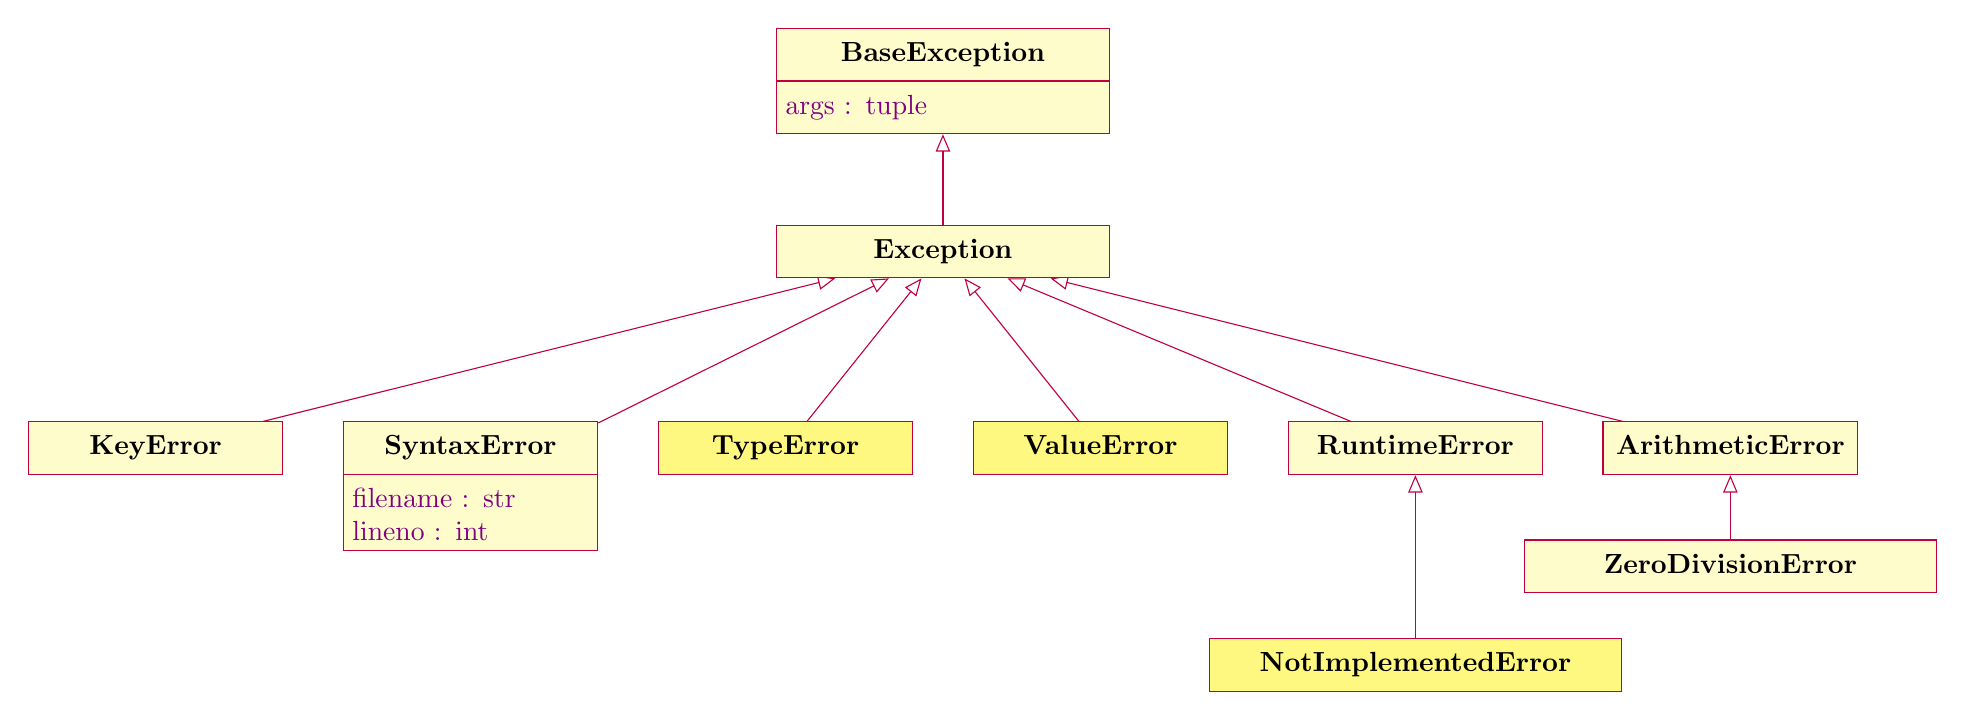
\begin{tikzpicture}

\begin{class}[text width=4cm, font=\strut]{BaseException}{0,0}
\operation{\attrcolor args : tuple}
\end{class}

\begin{class}[text width=4cm, font=\strut]{Exception}{0,-2.5}
\inherit{BaseException}
\end{class}

\begin{class}[text width=3cm, font=\strut]{SyntaxError}{-6,-5}
\inherit{Exception}
\attribute{\attrcolor filename : str}
\attribute{\attrcolor lineno : int}
\end{class}

\begin{class}[text width=3cm, font=\strut]{KeyError}{-10,-5}
\inherit{Exception}
\end{class}

\begin{class}[text width=3cm, font=\strut, fill=yellow!50]{TypeError}{-2,-5}
\inherit{Exception}
\end{class}

\begin{class}[text width=3cm, font=\strut, fill=yellow!50]{ValueError}{2,-5}
\inherit{Exception}
\end{class}

\begin{class}[text width=3cm, font=\strut]{RuntimeError}{6,-5}
\inherit{Exception}
\end{class}

\begin{class}[text width=3cm, font=\strut]{ArithmeticError}{10,-5}
\inherit{Exception}
\end{class}

\begin{class}[text width=5cm, font=\strut, fill=yellow!50]{NotImplementedError}{6,-7.75}
\inherit{RuntimeError}
\end{class}

\begin{class}[text width=5cm, font=\strut]{ZeroDivisionError}{10,-6.5}
\inherit{ArithmeticError}
\end{class}

\end{tikzpicture}
\end{document}
